\documentclass[12pt,compress]{beamer}
\usepackage{ifthen}

\title{Electron Identification \\ without the Pixel Detector}
\author{Jim Pivarski}
\institute{Cornell University}
\date{31 May, 2006}

\setbeamertemplate{navigation symbols}{}
\setbeamertemplate{headline}{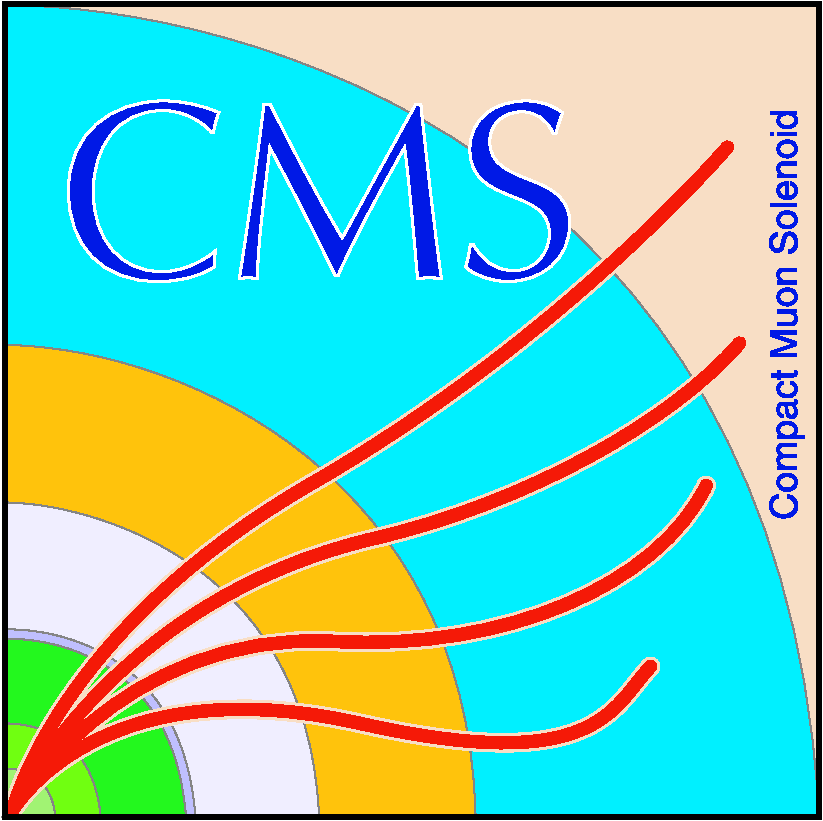
\includegraphics[height=1 cm]{cmslogo} \hfill
\begin{minipage}{8 cm}
\vspace{-0.75 cm} \small
\begin{center}
\ifthenelse{\equal{\insertpagenumber}{0}}{}{\insertsection\ (\insertpagenumber/\pageref{numpages})}
\end{center}
\end{minipage} \hfill 
\includegraphics[height=1 cm]{lepplogo}}

\xdefinecolor{verylightgray}{rgb}{0.95,0.95,0.95}
\beamertemplateshadingbackground{verylightgray}{white}

\begin{document}
\addtocounter{page}{-1}
\frame{\titlepage}
\section*{Pixelless Electrons --- Jim Pivarski}

\begin{frame}
\frametitle{Outline for this talk}

\begin{itemize}\setlength{\itemsep}{0.75 cm}
\item Project outline and goals
\item Disadvantages and advantages of electron-finding in the Si-strip tracker
\item The importance of realistic Monte Carlo
\item Status and next steps
\end{itemize}

\end{frame}

\begin{frame}
\frametitle{Project Outline and Goals}

\begin{description}
\item[Goal:] Identify electrons (HLT and offline) by matching ECAL
superclusters to Si-strip tracker hits
\end{description}

\begin{center}
\begin{tabular}{p{0.3\linewidth} p{0.3\linewidth} p{0.3\linewidth}}
\begin{minipage}{\linewidth} \begin{center} \textcolor{blue}{fast} \end{center} \end{minipage} & 
\begin{minipage}{\linewidth} \begin{center} \textcolor{blue}{robust} \end{center} \end{minipage} & 
\begin{minipage}{\linewidth} \begin{center} \textcolor{blue}{flexible} \end{center} \end{minipage} \\\hline
\begin{minipage}{\linewidth} \begin{center}

\vspace{0.25 cm} \small $\lesssim$ 100~ms per supercluster

\vspace{0.5 cm} $\mathcal{O}(\mbox{hits}\,^p)$ where $p \lesssim 2$
\end{center} \end{minipage} & 
\begin{minipage}{\linewidth} \begin{center}

\vspace{0.25 cm} \small $\epsilon$ indep.\ of misalignments

{\scriptsize ($\sim$500~$\mu$m in tracker, $\sim$1~mm tracker-ECAL)}

\vspace{0.5 cm} $\epsilon$ indep.\ of occupancy

\end{center} \end{minipage} &
\begin{minipage}{\linewidth} \begin{center}

\vspace{0.25 cm} \small provide parameters to tune

\vspace{0.25 cm} $\epsilon$ vs.\ rejection,

\vspace{0.25 cm} $\epsilon$ vs.\ speed

\end{center} \end{minipage}
\end{tabular}
\end{center}
\end{frame}

\begin{frame}
\frametitle{HLT Context: Level 2.5}

After ECAL clustering and before track-finding

\vfill
Provide a list of electron candidates: HLT should accept the event if \#candidates $>$ 0

\vspace{0.5 cm} {\scriptsize \color{blue} Level 2.0 $\rightarrow$ we insert
candidates into event $\rightarrow$ Level 2.5 Filter
$\rightarrow$ Level 3.0 tracking}

\vfill
Provide track parameters and possibly cloud of hits for Level 3.0 tracking
\end{frame}

\begin{frame}
\textcolor{blue}{\Large \hspace{-0.87 cm} Why it's harder without the Pixel detector}

\vspace{0.5 cm}
Pixel's 2D hits allow for a smaller search region (larger signal/noise)

\vspace{0.25 cm}
Pixel's resolution is 150~$\mu$m/$\sqrt{12}$, strip tracker's resolution is
\begin{itemize}
\item 1~mm/$\sqrt{12}$ in tracker's four stereo layers
\item 10--20~cm/$\sqrt{12}$ in segmented RPHI layers
\end{itemize}

\uncover<2>{
\vspace{0.5 cm}
\textcolor{blue}{\Large \hspace{-0.87 cm} Advantages of the Strip tracker}

\begin{itemize}
\item More layers: regain signal/noise with coincidence of hits
\item Hits close to and far from the ECAL\ldots
\end{itemize}}
\end{frame}

\begin{frame}
\frametitle{Two approaches to electron identification}

\begin{columns}
\column{0.45\linewidth}

{\bf Thm:} if electron and all bremsstrahlung photons are included
in a supercluster, energy-weighted position is on the initial helix

\column{0.45\linewidth}
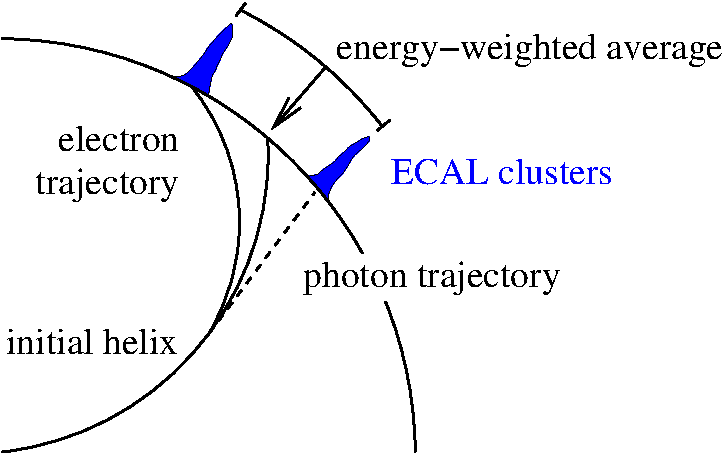
\includegraphics[width=\linewidth]{theorem}

\end{columns}

\vfill
Two approaches to hit matching:
\begin{itemize}
\item Inner hits point to supercluster position
\item Outer hits point to a basiccluster position
\end{itemize}

The two approaches may be combined
\end{frame}

\begin{frame}
\frametitle{``Event Displays''}

\begin{itemize}
\item vertical axis is $\phi$ of each hit with supercluster's $\phi$ as zero
\item horizontal axis is cylindrical radius of each hit
\end{itemize}

\begin{center}
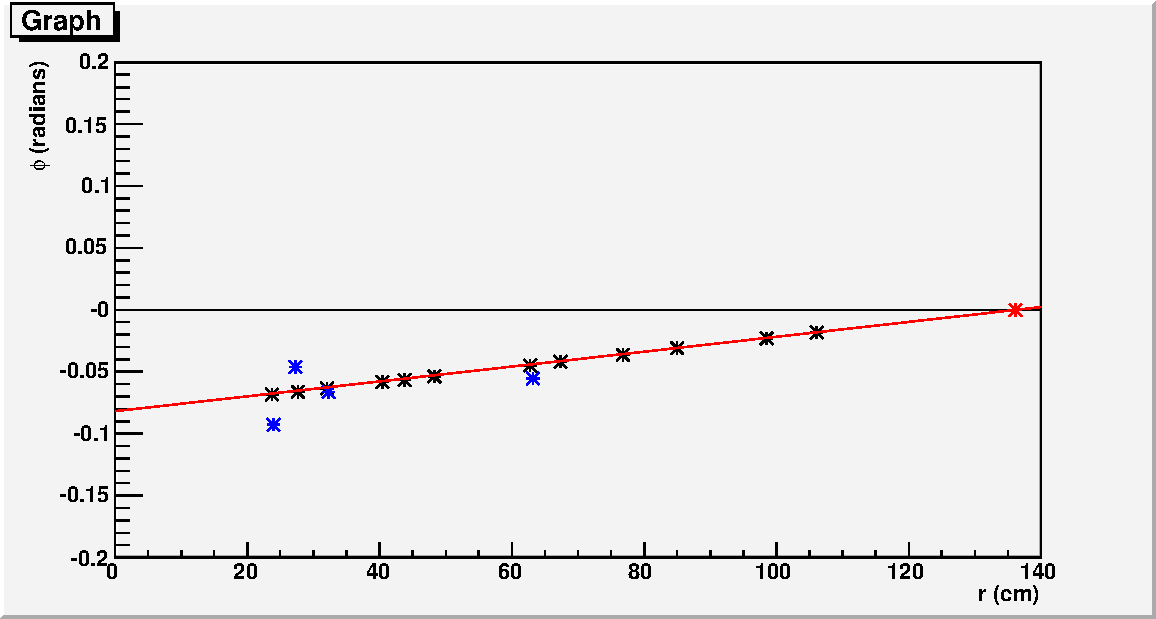
\includegraphics[width=0.85\linewidth]{event_display}
\end{center}

\end{frame}

\begin{frame}
\frametitle{Electron pathologies}

\vspace{-1 cm}
\begin{center}
\begin{tabular}{p{0.55\linewidth} p{0.4\linewidth}}
\begin{minipage}{\linewidth} Scatter before tracker ($\sim$4\%) \end{minipage} &
\begin{minipage}{\linewidth} 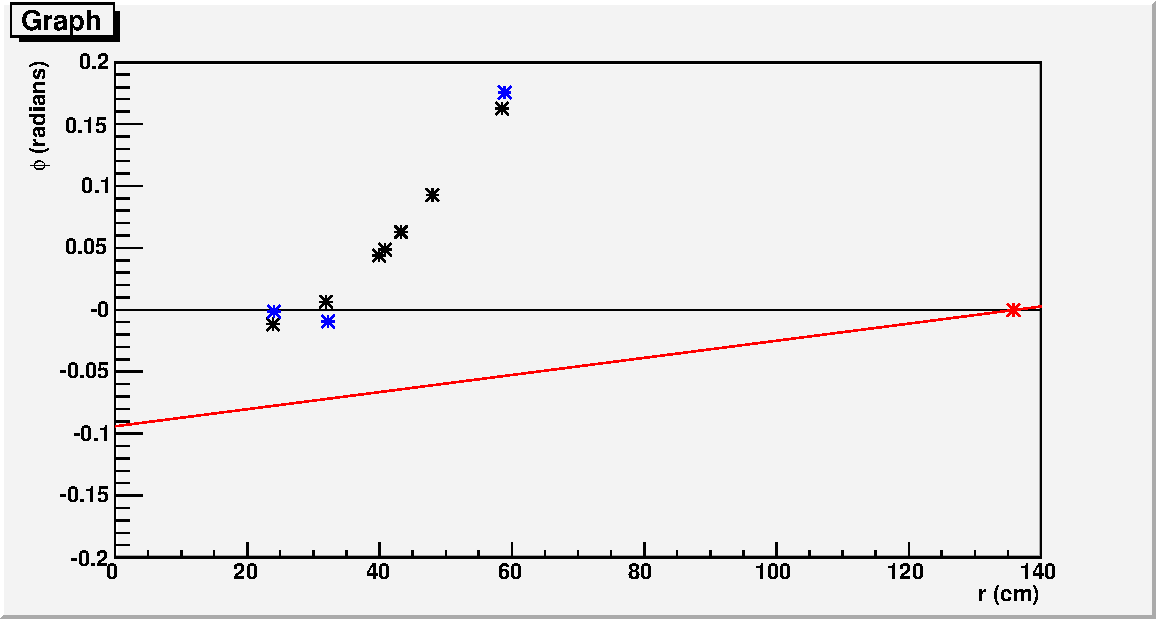
\includegraphics[width=\linewidth]{event_display_scatterearly} \end{minipage} \\
\begin{minipage}{\linewidth} Scatter in tracker ($\sim$4\%) \end{minipage} &
\begin{minipage}{\linewidth} 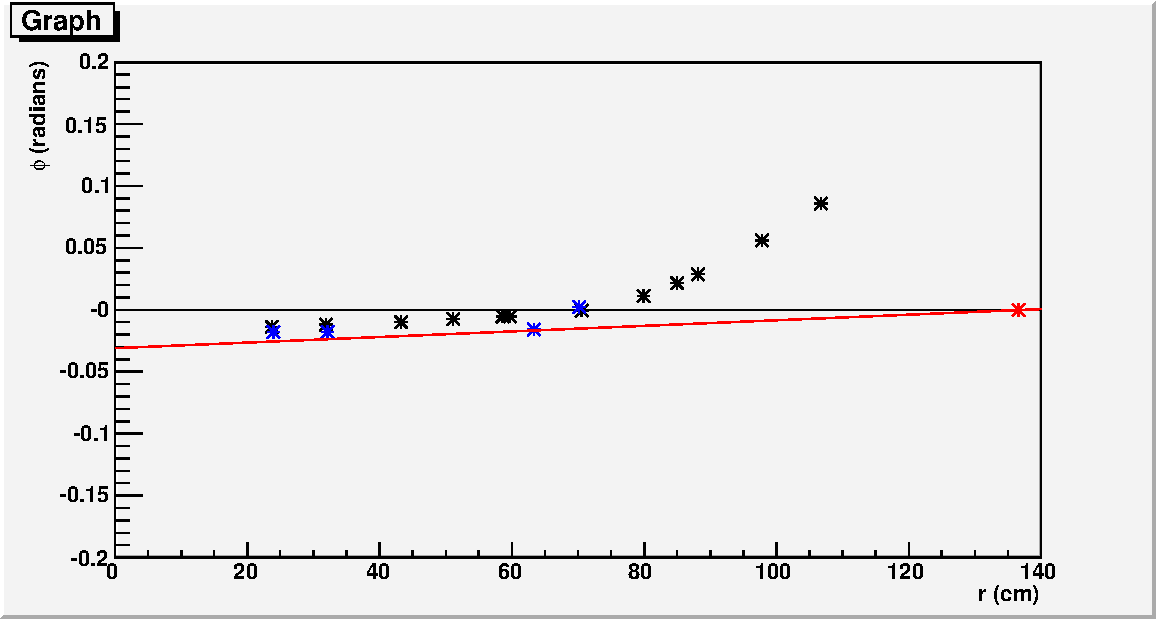
\includegraphics[width=\linewidth]{event_display_scattersi2} \end{minipage} \\
\begin{minipage}{\linewidth} Wrong supercluster position \\ ($\sim$12\% at 10~GeV) \end{minipage} &
\begin{minipage}{\linewidth} 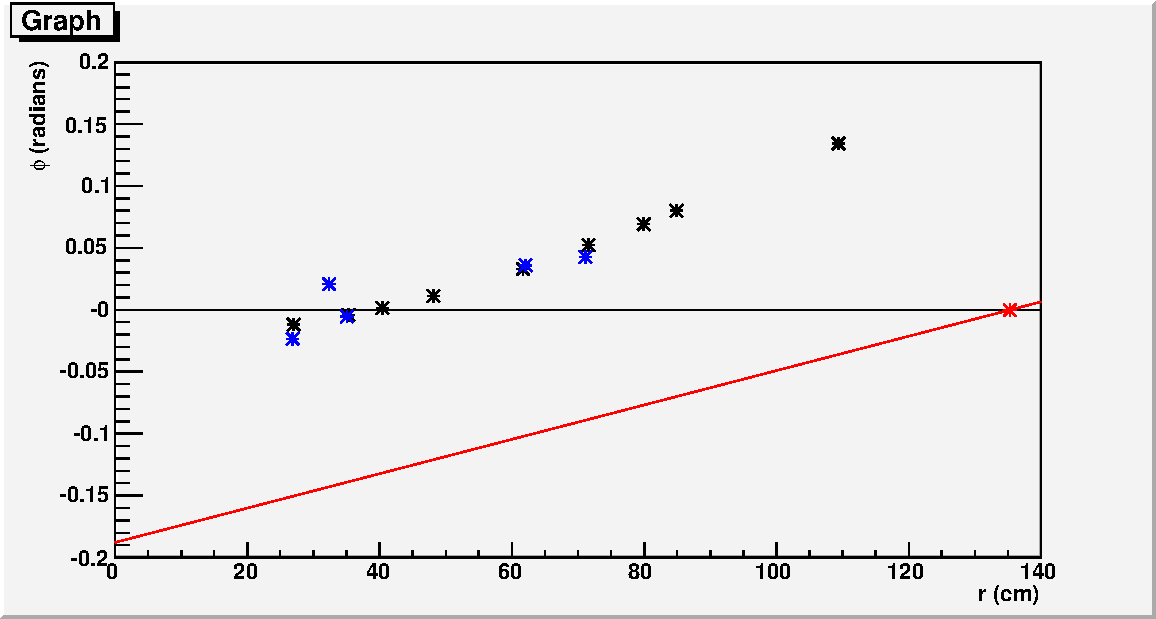
\includegraphics[width=\linewidth]{event_display_wrongsc} \end{minipage} \\
\end{tabular}
\end{center}

\end{frame}

\begin{frame}
\frametitle{Typical occupancy (superimposed minbias event)}

\begin{center}
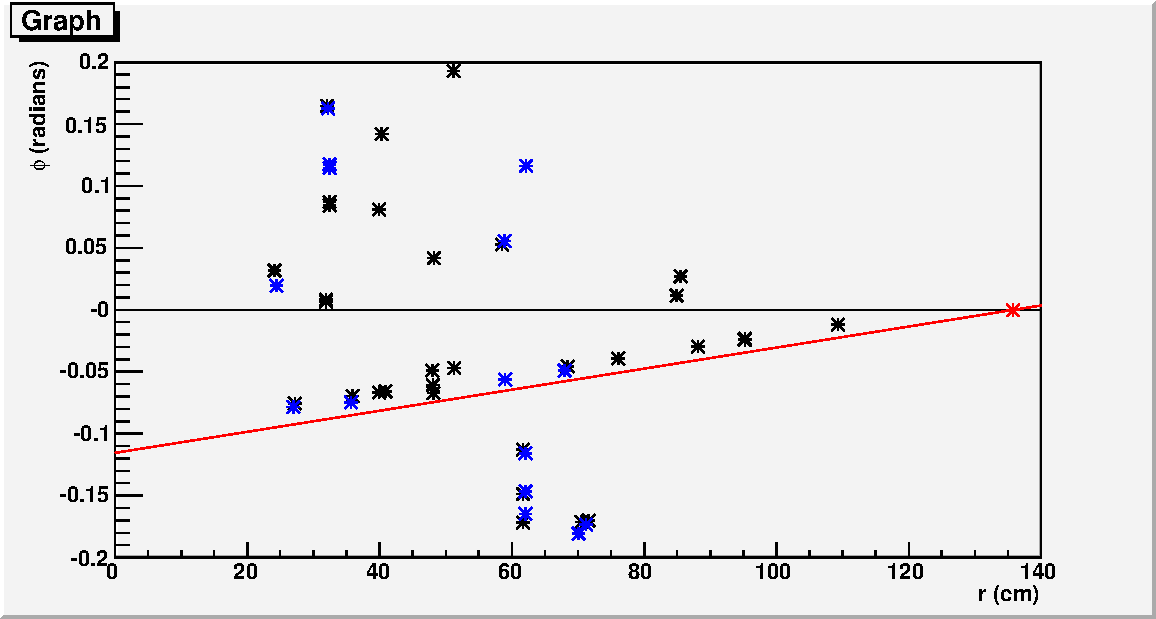
\includegraphics[width=\linewidth]{event_display_superimposed}
\end{center}
\end{frame}

\begin{frame}
\frametitle{Background: minbias \underline{with a 17~GeV supercluster}} % 17.8 GeV

\begin{center}
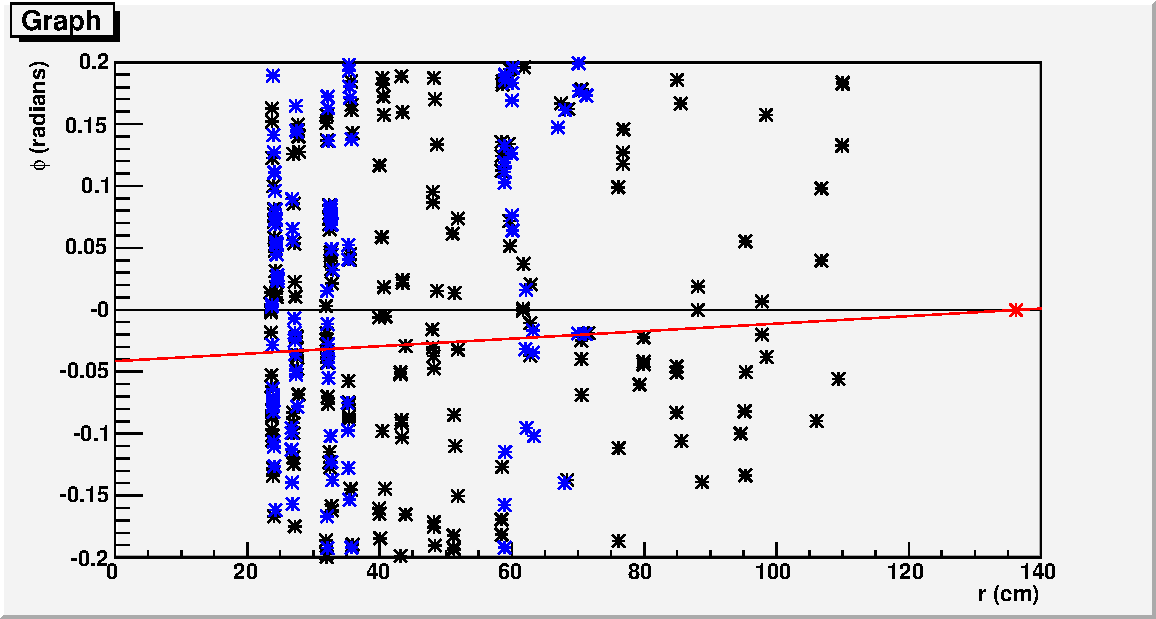
\includegraphics[width=\linewidth]{event_display_background}
\end{center}
\end{frame}

\begin{frame}
\frametitle{Analysis of a simple algorithm}

Define a 10~mrad $\Delta \phi$ band around hypothesis, count hits within that band

\begin{center}
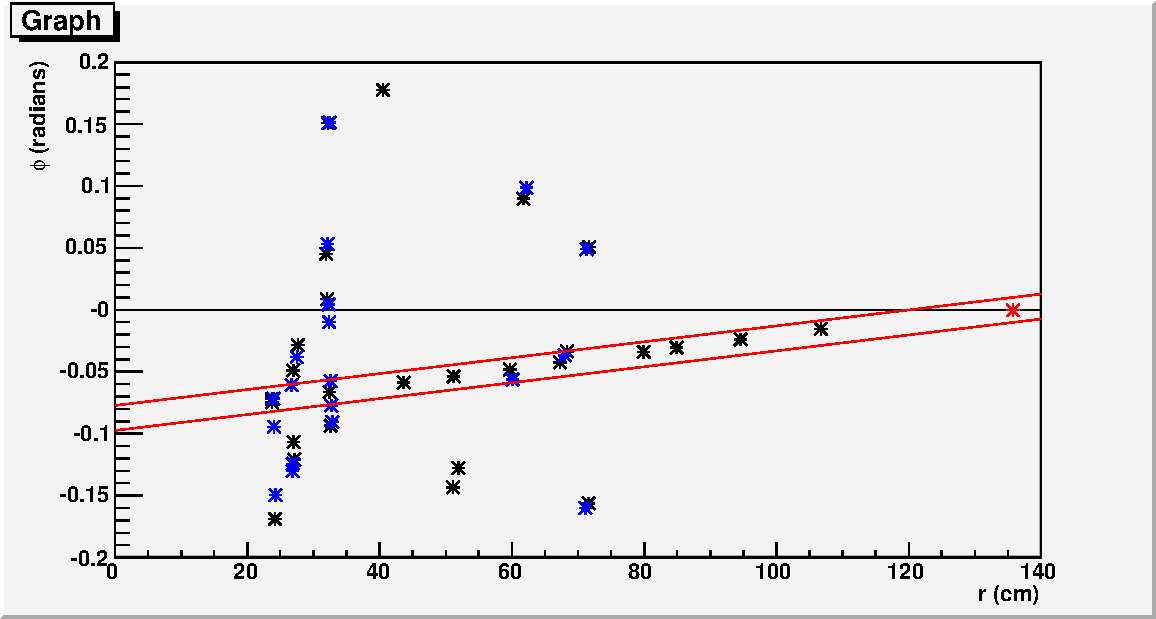
\includegraphics[width=0.9\linewidth]{event_display_banded}
\end{center}
\end{frame}

\begin{frame}
Good discrimination between \textcolor{red}{electrons} and minbias,

poor discrimination between \textcolor{red}{electrons} and \textcolor{blue}{minbias passing L1}

\begin{center}
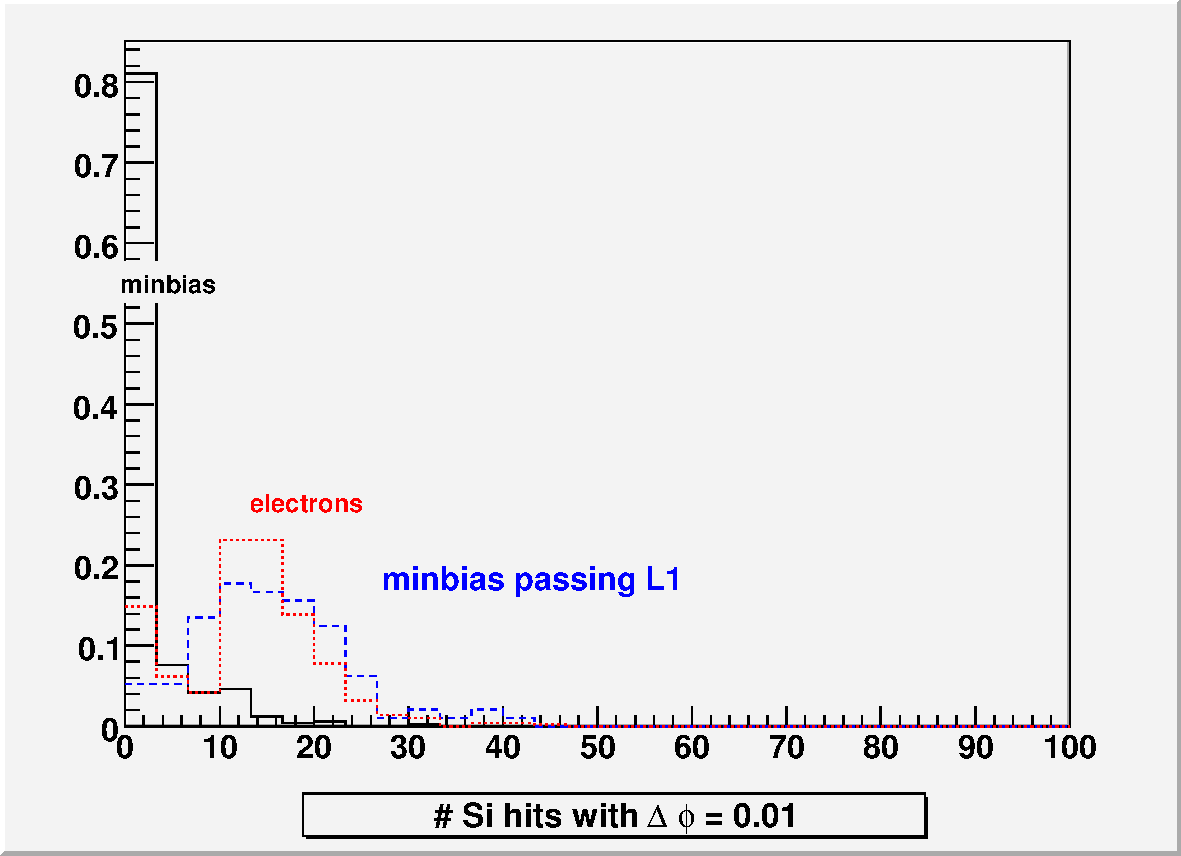
\includegraphics[width=0.65\linewidth]{hitdistributions}
\end{center}

\textcolor{blue}{minbias passing L1} ($\ge$~17~GeV supercluster) points into a jet
\end{frame}

\begin{frame}
Narrow $\Delta \phi$ to 2~mrad?

\begin{center}
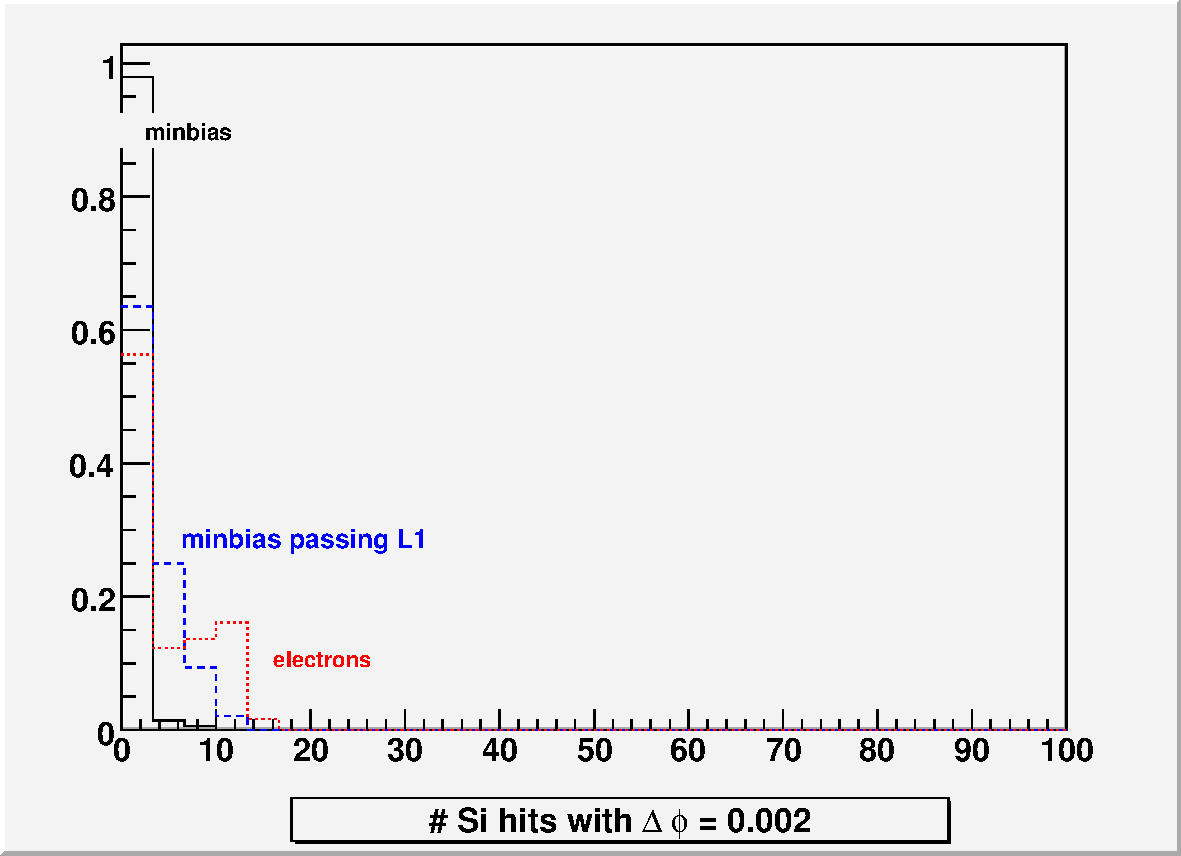
\includegraphics[width=0.65\linewidth]{hitdistributions_narrow}
\end{center}

Not narrow enough to distinguish electrons from background,

and too narrow for robustness goals
\end{frame}

\begin{frame}
Widen $\Delta \phi$ to 100~mrad and cut on {\it maximum} number of hits?

\begin{center}
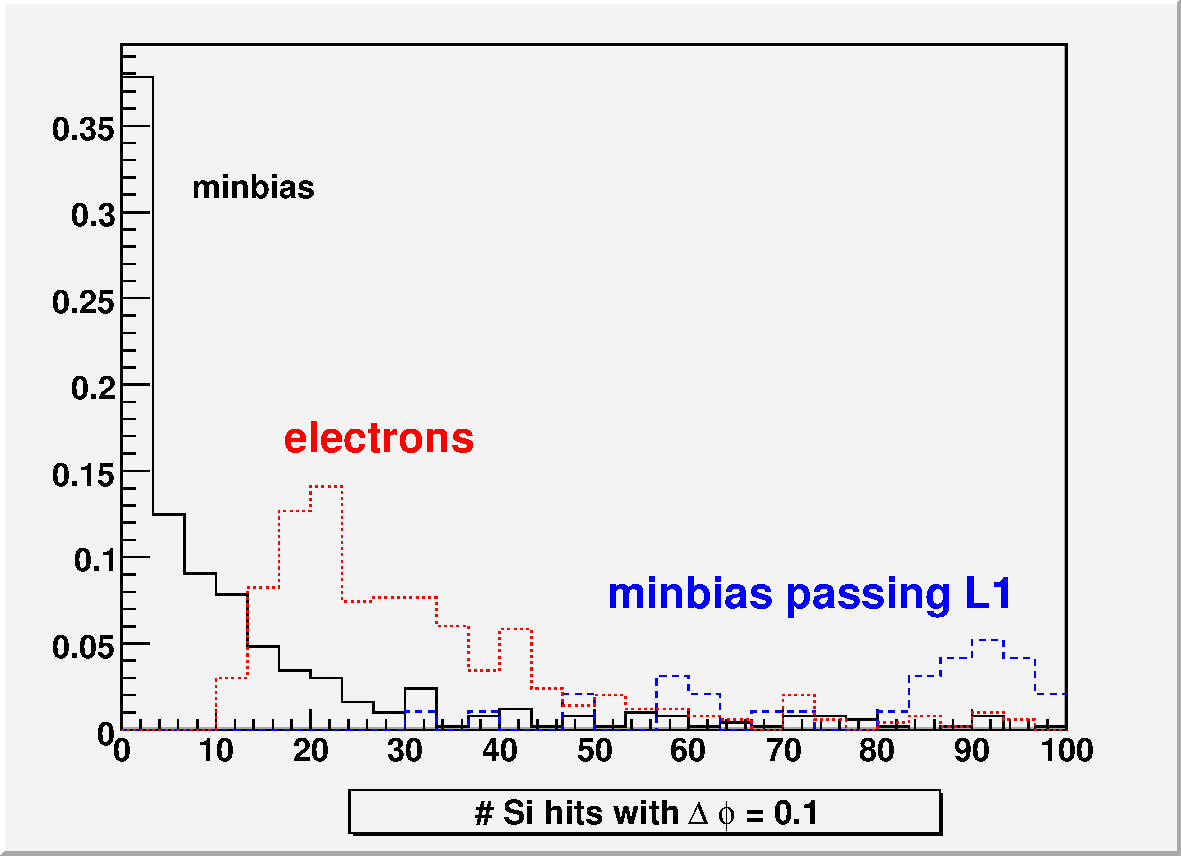
\includegraphics[width=0.65\linewidth]{hitdistributions_wide}
\end{center}

That would be a track isolation cut, not track matching!

Can we afford to isolate electons?

\begin{center}
\textcolor{blue}{\fbox{MC studies drive algorithm development}}
\end{center}
\end{frame}

\begin{frame}
\textcolor{blue}{\Large \hspace{-0.87 cm} Status}
\begin{itemize}
\item Performed informal first studies of signal and background
\item Implemented placeholder {\tt SiStripElectronCandidate} and
{\tt SiStripElectronProducer} in {\tt CMSSW\_0\_7\_0\_pre2}
\end{itemize}

\vfill
\textcolor{blue}{\Large \hspace{-0.87 cm} Next Steps}
\begin{enumerate}
\item Obtain realistic Monte Carlo
\begin{description}
\item[signal:] physics electrons (jet overlap?)

superimpose hadronic background at the generator level

\item[background:] large minbias sample which has passed L2

\end{description}

\item Study event properties (in CMSSW/FWLite)

\hspace{2.5 cm} $\uparrow$ \hspace{0.5 cm} $\downarrow$

\item Improve algorithm (in CMSSW)
\end{enumerate}

\label{numpages}
\end{frame}

\end{document}
